%% Appendix B: Mechanical Diagram Gallery

\section*{Subsystem Visualization}

This appendix contains detailed mechanical diagrams referenced throughout the whitepaper.

\subsection*{System Architecture}

%% System Architecture Diagram
%% Five primary subsystems of the Babbage Analytical Engine

\begin{tikzpicture}[scale=1.2, node distance=2cm]

% Define subsystem blocks
\node[block, fill=blue!10, minimum width=2.5cm] (mill) {The Mill\\(Arithmetic Unit)};
\node[block, fill=green!10, right=3.5cm of mill, minimum width=2.5cm] (store) {The Store\\(Memory)};
\node[block, fill=yellow!10, below=3cm of mill, minimum width=2.5cm] (barrel) {The Barrel\\(Control)};
\node[block, fill=purple!10, below=3cm of store, minimum width=2.5cm] (io) {Input/Output\\(I/O)};
\node[block, fill=red!10, right=3.5cm of barrel, minimum width=2.5cm] (seq) {Sequencer\\(Processes)};

% Central coordination point
\node[circle, draw=black, thick, fill=white, inner sep=0.3cm] (center) at (1.25,-1.5) {System Bus};

% Draw connections from each subsystem to center
\draw[thick, ->] (mill) -- (center);
\draw[thick, ->] (store) -- (center);
\draw[thick, ->] (barrel) -- (center);
\draw[thick, ->] (io) -- (center);
\draw[thick, ->] (seq) -- (center);

% Add labels for data paths
\node[font=\small, above=0.1cm] at (0.5,-0.8) {50-bit data};
\node[font=\small, above=0.1cm] at (2,-0.8) {11-bit addr};
\node[font=\small, above=0.1cm] at (0.5,-2.2) {Control};
\node[font=\small, above=0.1cm] at (2,-2.2) {Process};

% Add subsystem descriptions
\node[font=\tiny, below=0.8cm of mill, text width=2.2cm, align=center] {Performs ADD, SUB, MUL, DIV on 50-digit decimals};
\node[font=\tiny, below=0.8cm of store, text width=2.2cm, align=center] {2,000 × 50 digit matrix, 15s access time};
\node[font=\tiny, below=0.8cm of barrel, text width=2.2cm, align=center] {Pegged cylinder, 32-instruction ISA};
\node[font=\tiny, below=0.8cm of io, text width=2.2cm, align=center] {Cards, printer, communication};
\node[font=\tiny, below=0.8cm of seq, text width=2.2cm, align=center] {Round-robin, 67 processes};

% Add operating frequency annotation
\node[font=\small, below=5cm] at (1.25,-5) {Operating frequency: $\sim$1 instruction per 8--750 seconds};
\node[font=\small, below=5.5cm] at (1.25,-5) {(Depends on operation complexity)};

\end{tikzpicture}


Five primary subsystems connected via central system bus: Mill (arithmetic), Store (memory), Barrel (control), I/O, and Sequencer (process management).

\subsection*{Carry Propagation Mechanism}

%% Carry Propagation Mechanism
%% Shows how carries cascade through digit positions during arithmetic

\begin{tikzpicture}[scale=1.0]

% Draw 5 digit positions (0-4)
\foreach \i in {0, 1, 2, 3, 4} {
    \coordinate (digit-\i) at (\i * 2, 0);
    \node[circle, draw=black, thick, fill=white, minimum size=1.2cm] at (digit-\i) {\small Digit \i};
    
    % Draw gear representation (12mm gear with 10 positions)
    \draw[very thin, gray] (digit-\i) circle (0.5cm);
    
    % Show digit position (0-9)
    \node[font=\tiny, above=0.6cm of digit-\i] (pos-\i) {Position: 0--9};
}

% Draw carry propagation arrows
\foreach \i in {0, 1, 2, 3} {
    \pgfmathsetmacro\j{\i + 1}
    \draw[->, thick, red] ($(digit-\i) + (0.6, 0)$) -- ($(digit-\j) + (-0.6, 0)$);
    \node[font=\small, red, above=0.2cm] at ($(digit-\i) + (1, 0)$) {Carry};
}

% Show example: 999 + 1 = 1000 (carry propagation)
\node[below=3cm, font=\large\bfseries] at (4, 0) {Example: 9 + 1 = 10 (carry cascades)};
\node[below=3.5cm, font=\footnotesize, text width=8cm, align=center] at (4, 0) {
    When digit 0 reaches 10, pawl engages digit 1, incrementing it.\\
    If digit 1 already at 9, carry cascades through digit 2, 3, 4, etc.
};

% Draw mechanical implementation detail
\draw[very thin, dashed] (0, -2) -- (8, -2);
\node[below=-1.8cm, font=\small] at (0, -2) {Mechanical Implementation:};

\draw[thick] (0.5, -2.5) rectangle (1.5, -3.5);
\node[font=\tiny, align=center] at (1, -3) {Digit\\wheel};

\draw[thick, ->] (1.5, -3) -- (2, -3);
\node[font=\tiny, above=0.1cm] at (1.75, -2.9) {Pawl};

\draw[thick] (2, -2.5) rectangle (3, -3.5);
\node[font=\tiny, align=center] at (2.5, -3) {Next\\digit};

% Annotation
\node[font=\footnotesize, below=0.5cm] at (4, -4) {Carry time: $\sim$0.5 seconds per digit position};

\end{tikzpicture}


Mechanical cascade mechanism enabling addition/subtraction across 50 digit positions. Pawls engage sequentially during carry propagation.

\subsection*{Memory Store Organization}

%% Store Memory Organization
%% 2,000 x 50 digit matrix with address decoding

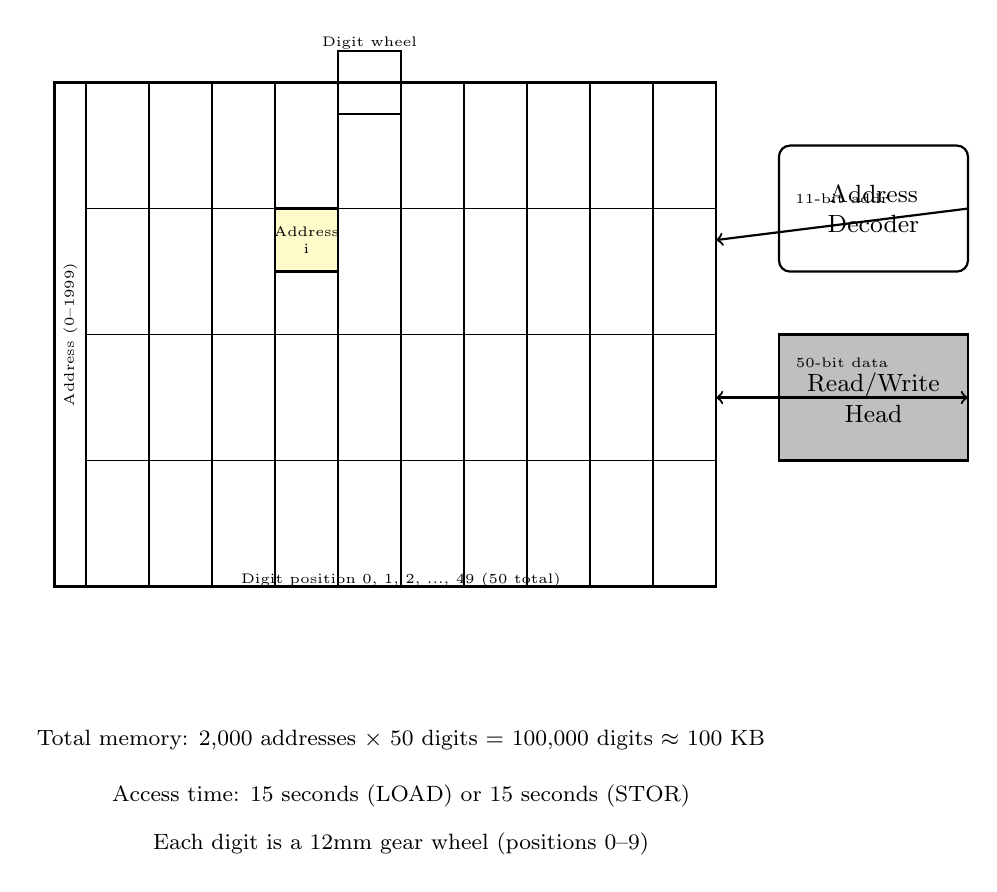
\begin{tikzpicture}[scale=0.8]

% Draw memory matrix (simplified)
\draw[thick] (0, 0) rectangle (10, 8);

% Draw address on left
\draw[thick] (-0.5, 0) rectangle (0, 8);
\node[font=\tiny, rotate=90, align=center] at (-0.25, 4) {Address (0--1999)};

% Draw columns for digit positions (50 total, show 10)
\foreach \i in {0, 1, 2, ..., 9} {
    \draw[thin] (\i, 0) -- (\i, 8);
}
\node[font=\tiny, below=-0.3cm] at (5, 0) {Digit position 0, 1, 2, ..., 49 (50 total)};

% Draw some rows
\foreach \row in {0, 2, 4, 6} {
    \draw[thin] (0, \row) -- (10, \row);
}

% Highlight one memory location
\draw[thick, fill=yellow!20] (3, 5) rectangle (4, 6);
\node[font=\tiny, align=center] at (3.5, 5.5) {Address\\i};

% Draw address decoder
\draw[thick, rounded corners] (11, 5) rectangle (14, 7);
\node[font=\small, align=center] at (12.5, 6) {Address\\Decoder};

% Draw connection from decoder to memory
\draw[thick, ->] (14, 6) -- (10, 5.5);
\node[font=\tiny, above=0.1cm] at (12, 5.8) {11-bit addr};

% Draw read/write mechanism
\draw[thick, fill=lightgray] (11, 2) rectangle (14, 4);
\node[font=\small, align=center] at (12.5, 3) {Read/Write\\Head};

% Draw connection to memory location
\draw[thick, <->] (14, 3) -- (10, 3);
\node[font=\tiny, above=0.1cm] at (12, 3.2) {50-bit data};

% Memory organization annotation
\node[font=\footnotesize, below=0.5cm] at (5, -1.5) {Total memory: 2,000 addresses $\times$ 50 digits = 100,000 digits $\approx$ 100 KB};
\node[font=\footnotesize, below=1.2cm] at (5, -1.5) {Access time: 15 seconds (LOAD) or 15 seconds (STOR)};

% Show data format in one cell
\draw[thick] (4, 7.5) rectangle (5, 8.5);
\node[font=\tiny, above=-0.1cm] at (4.5, 8.5) {Digit wheel};
\node[font=\footnotesize, below=1.8cm] at (5, -1.5) {Each digit is a 12mm gear wheel (positions 0--9)};

\end{tikzpicture}


2,000 × 50 matrix memory with address decoding and read/write mechanisms. Each digit wheel is a 12mm gear with 10 positions (0--9).

\subsection*{Process Control Block Layout (Table Form)}

See Table \ref{tab:pcb-layout} in Section \ref{sec:unix-mapping} for detailed PCB structure.

\subsection*{Pipe Buffer Implementation}

The pipe mechanism uses a rotating 8-slot drum with independent read/write pointers. Each slot stores one 50-digit number. Mechanical engagement detects empty/full conditions and blocks reader/writer as appropriate.

\subsection*{Digit Wheel Assembly}

Each digit wheel is a precisely cut gear:
\begin{itemize}
    \item Diameter: 12 mm
    \item Material: Hardened steel
    \item Number of teeth: 10 (representing digits 0--9)
    \item Tolerance: ±0.15 mm (hobbing accuracy)
    \item Mounting: Press-fit onto shaft
\end{itemize}

\subsection*{Bearing Configuration}

Two bearing types used throughout:
\begin{itemize}
    \item Timken roller bearings (high-speed drives): Superior load rating, lower friction
    \item Bronze journal bearings (low-speed): Cost-effective, adequate for carry mechanisms
\end{itemize}

\subsection*{Assembly Integration Points}

Key interfaces between subsystems:
\begin{enumerate}
    \item Mill output to Store write-path
    \item Store read-path to Mill input
    \item Barrel to Mill (opcode lines)
    \item Barrel to Sequencer (process control)
    \item I/O devices to Store (card data buffering)
\end{enumerate}

